\documentclass[article]{aaltoseries}
\usepackage[utf8]{inputenc}


\begin{document}
 
%=========================================================

\title{Comparison of theorem provers}

\author{Artem Yushkovskiy
\\\textnormal{\texttt{artem.yushkovskiy@aalto.fi}}}

\affiliation{\textbf{Tutor}: Stavros Tripakis}

\maketitle

%==========================================================

\begin{abstract}
One of the useful applications mathematical logic theory is the Automated theorem proving. This is a set of techniques that allow one to verify mathematical statements mechanically using logical reasoning. Although, it can be also used to solve engineering problems, for instance to prove security properties for a software system or an algorithm. Furthermore, automated theorem proving is an essential part of the Artificial Intelligence theory, which became highly evolving these days. In this paper, we describe bases of formal systems and automated deduction theory, and compare two widespread tools for automated theorem proving, Coq [1] and Isabelle [2].

\vspace{3mm}
\noindent KEYWORDS: logic, automated theorem prover, Coq, Isabelle

\end{abstract}


%============================================================


\section{Introduction}

In general terms, \textit{formal proof} is the sequence of statements, based on finite set of fundamental axioms and satisfying the rules of logical inference. \textit{The axiom} is a statement claimed to be true evidently. \textit{The logical inference} is the transfer from one statement (premise) to another (consequence), which preserve truth, while the rule of logical inference is a principle that allows one to infer the validity of such transfer. In formal logic, inference is based entirely on the structure (i.e., form) of those statements, which allows one to apply basic logical rules to any type of proof and thus construct the formal system.

The main goal of the formal system is to be verifiable, i.e. one could \textit{check} its validity. At present, a lot of tools are being developing to automate the process of such checking to run it on the computer. In particular, the systems \textit{Isabelle/ZF}~[???], \textit{Coq}~[???], PVS~[???], ACL~[???] work in a form of axiomatic set theory and allow the user to enter theorems and proofs into the computer, which then verifies that the proof is correct (these are also called sometimes "proof assistants").
Another goal of constructing the formal system is having the computer to \textit{discover} formal proof. This goal is different from the previous one since the system must be optimised for efficient search. The output proofs can rely on induction, or on meta argument, or on higher-order logic. McCune’s systems \textit{Otter}~[???] and \textit{Prover9}~[???] are commonly recognized as the state-of-the-art tools~[Com00].

In current paper we consider only the systems, which are built to achieve the first goal, i.e. to verify existing proof, since <...>. Two aforementioned theorem provers Coq and Isabelle are examined for the purpose of revealing expressiveness, computation power and usability. These properties are described in detail in section <???>. Section~\ref{sec:formal_theory} gives an overview of the history of logic providing thorough definitions, typology and properties of formal system and formal proof. Issues related to theoretical limitations of formal systems are discussed further as well. <... about comparison, results and author's personal contrubution>

%============================================================

\section{Theory of logical calculi}
\label{sec:formal_theory}
// TODO

set theory, Zermelo–Fraenkel, briefly 1st and 2nd ordered logic, 

an example from wiki: A formal system or logical calculus is any well-defined system of abstract thought based on the model of mathematics. A formal system need not be mathematical as such; for example, Spinoza's Ethics imitates the form of Euclid's Elements. Spinoza employed Euclidiean elements such as "axioms" or "primitive truths", rules of inferences etc. so that a calculus can be built using these. For nature of such primitive truths, one can consult Tarski's "Concept of truth for a formalized language".

%============================================================

\subsection{History of logic calculi}
\label{sec:history}
// TODO

A long time ago in a galaxy far, far away...

Hilbert's programme, ...

Mock text from wiki: %https://en.wikipedia.org/wiki/History\_of\_logic#Traditional\_logic:
\begin{itemize}
	
	\item The embryonic period from Leibniz to 1847, when the notion of a logical calculus was discussed and developed, particularly by Leibniz, but no schools were formed, and isolated periodic attempts were abandoned or went unnoticed.
	
	\item The algebraic period from Boole's Analysis to Schröder's Vorlesungen. In this period, there were more practitioners, and a greater continuity of development.
	
	\item The logicist period from the Begriffsschrift of Frege to the Principia Mathematica of Russell and Whitehead. The aim of the "logicist school" was to incorporate the logic of all mathematical and scientific discourse in a single unified system which, taking as a fundamental principle that all mathematical truths are logical, did not accept any non-logical terminology. The major logicists were Frege, Russell, and the early Wittgenstein.[92] It culminates with the Principia, an important work which includes a thorough examination and attempted solution of the antinomies which had been an obstacle to earlier progress.
	
	\item The metamathematical period from 1910 to the 1930s, which saw the development of metalogic, in the finitist system of Hilbert, and the non-finitist system of Löwenheim and Skolem, the combination of logic and metalogic in the work of Gödel and Tarski. Gödel's incompleteness theorem of 1931 was one of the greatest achievements in the history of logic. Later in the 1930s, Gödel developed the notion of set-theoretic constructibility.
	The period after World War II, when mathematical logic branched into four inter-related but separate areas of research: model theory, proof theory, computability theory, and set theory, and its ideas and methods began to influence philosophy.
	
\end{itemize}






%============================================================

\subsection{Limitations of logic systems}
\label{sec:limitations}
// TODO

first-order logic

%------------------------------------------------------------


\subsection{Emphasizing text}
\label{sec:emphasis}

\textit{Italics} is a good way to emphasize printed text. However,
\textbf{boldface} looks better when converted to HTML.

Paragraphs are separated by an empty line in the Latex source code.
Latex puts extra space between sentences, which you must suppress
after a period that does not end a sentence, e.g.\ after this acronym.

Cross-references to figures (Fig.~\ref{fig:mypicture1}), tables
(Table~\ref{tab:mytable1}), other sections (Sec.~\ref{sec:math})
are easy to create. 


%------------------------------------------------------------


\subsection{Mathematics}
\label{sec:math}

In the mathematics mode, you can have subscripts such as $K_{master}$
and superscripts like $2^x$. Longer formulas may be put on a separate
line:
\[ \emptyset \in \emptyset \; \Rightarrow \; E \neq mc^2. \]

You may also want to number the formulas like Eq.~(\ref{eqn:myequation1})
below.
\begin{equation}\label{eqn:myequation1}
C = E_{K_{public}}(P) = P^e. \hspace{10mm}   P = D_{K_{private}}(C) = C^d.
\end{equation}



%------------------------------------------------------------


\subsection{Make a list}
\label{sec:list}

Lists can have either bullets or numbers on them. 

\begin{itemize}
\item one item
\item another item, which is an exceptionally long one for an item
  and consequently continues on the next line.
\end{itemize}

Lists can have several levels. Item~\ref{kukkuu} below contains
another list.
\begin{enumerate}
\item the fist item \label{kukkuu}
  \begin{enumerate}
  \item the first subitem 
  \item the second subitem
  \end{enumerate}
\item the second item
\end{enumerate}


%============================================================


\section{More complex stuff}

This section provides examples of more complex things.


%------------------------------------------------------------


\subsection{Data served on a table}


Table~\ref{tab:mytable1} presents some data in tabular form. 

\begin{table}[t!]
  \begin{center}
    \begin{tabular}{|l|lr|}
    \hline
    Protocol & Year &  RFC \\
    \hline
    TCP      & 1981 &  793 \\
    ISAKMP   & 1998 & 2408 \\
    Photuris & 1999 & 2522 \\
    \hline
    \end{tabular}
    \caption{A table with some protocols}
    \label{tab:mytable1}
  \end{center}
\end{table}


%------------------------------------------------------------


\subsection{Adding references}
\label{sec:references}

Do not forget to give pointers to the literature. If you are listing
stuff related to your topic, you can give several references once
\cite{Com00,HTS03,Nik99}. However, usually you should give only one, for example the standard describing the stuff \cite{RFC2408} and if you want to directly use someone else's words, use both quotation marks and refer to the source, for example that ``the developer does not need to know all about the framework to develop a working implementation'' \cite{Suo98}. Remember also to mark references to your pictures if they are not created by your own mind!

If you plan to write with Latex regularly, create your own BibTeX
database and use BibTeX to typeset the bibliographies automatically.
In the long run, it will save you a lot of time and effort compared to
compiling reference lists by hand.


%------------------------------------------------------------


\subsection{Embedded pictures}
\label{sec:pictures}

Fig.~\ref{fig:mypicture1} is an embedded picture. The supported formats for pictures
depend on the actual LaTeX command used. For instance, regular \LaTeX supports
pictures in EPS (Embedded PostScript) format, while pdf\LaTeX supports PDF (Portable
Document Format), PNG (Portable Network Graphics) and JPEG (Joint Photographic Experts
Group). It is recommended to use either EPS or PDF for diagrams as well as for any picture
which includes vector images.

\begin{figure}[t!]
  \begin{center}
    % Note how the file extension has been removed from the filename below
    % so that the LaTeX command can automatically pick any supported file format
    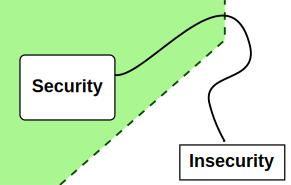
\includegraphics[width=.5\textwidth]{figures/sample}
    \caption{An embedded picture}
    \label{fig:mypicture1}
  \end{center}
\end{figure}


%============================================================


\section{Yet another section title}

To be added.


%============================================================


\section{Conclusion}

To be added.


%============================================================


\bibliographystyle{plain}
\bibliography{cs-seminar}

\end{document}
